% ########################################

\chapter{Conclusions and Future Work}
\label{chap:conclusion}

% ~~~~~~~~~~~~~~~~~~~~

\chaptoc{}

% ########################################

\section{Summary and Conclusions}
\label{sec:conclusion}

% ~~~~~~~~~~~~~~~~~~~~

\begin{colsection}

In this thesis I have described my work as part of the GOTO project, primarily working on the control software in order to create a fully-autonomous robotic telescope. After several years of development and commissioning the prototype GOTO telescope is fully operational, and observing from La Palma most nights with no human interaction.

\end{colsection}

% ~~~~~~~~~~~~~~~~~~~~

\subsection{Telescope control}
\label{sec:control_results}
\begin{colsection}

The core of my work has been the \acro{gtecs}, a Python software package that controls every aspect of the telescope. The hardware control daemons interface with the dome, mount and cameras (see \aref{chap:gtecs}) while the ``pilot'' master control program and its associated systems allow the telescope to function with no human involvement (see \aref{chap:autonomous}). GOTO has now been operating successfully for years with the pilot in full control. The conditions monitoring systems have proven robust enough to trust the dome to close in bad weather, and when the occasional unexpected hardware issues do occur the pilot recovery systems can fix the problem and resume observing in the majority of cases, often before a human even has time to log in. Of course, commissioning was not entirely without incident, as described in \aref{chap:commissioning}. However all of the software challenges were overcome, and the majority of the delays to GOTO were due to hardware faults which were out of my purview.

Each set of exposures taken with the G-TeCS camera daemon are assigned an incremental run number. From the initial installation in the summer of 2017 up until September 2019, GOTO had taken over 185,000 such exposure sets, and produced many tens of terabytes of data. The current all-sky survey that began in February 2019 has almost completely covered the northern sky, and at the time of writing the GOTO photometry database contains approximately 642 million sources from almost 500,000 individual frames taken since the start of the survey.

\newpage

\end{colsection}

% ~~~~~~~~~~~~~~~~~~~~

\subsection{Scheduling and alert follow-up}
\label{sec:gw_results}
\begin{colsection}

As outlined in \aref{sec:control_requirements}, GOTO needed an observation scheduling system that could deal with both the survey and gravitational-wave follow-up modes. The scheduler used by G-TeCS is a just-in-time system (see \aref{chap:scheduling}), where the highest priority target is recalculated every time the scheduler is called. This makes it very reactive to transient alerts, which was a requirement of the project.

As previously detailed in \aref{sec:gw_detections}, in the first 5 months of the third LIGO-Virgo observing run (O3) 32 gravitational-wave events were detected, all predicted to come from compact binary mergers. These events are listed in \aref{tab:gw_log}. Of the 32 alerts 7 were ultimately retracted by the LVC, leaving 25 real events, and only three of these (S190425z, S190426c and S190814bv) are thought to have originated from sources that could produce visible optical counterparts (binary neutron stars or neutron star-black hole binaries). However, events are currently infrequent enough for GOTO to react to all of them, even if there was a very low chance of there being a visible counterpart.

The G-TeCS sentinel received and reacted to every one of these alerts. In a few cases the event handler initially failed to process the VOEvent or the skymap, as described in \aref{sec:challenges}; this was usually due to a problem on the LVC end, and, after each time, changes were made to the GOTO-alert code to work around the problem should it happen again. For every alert the sentinel received the VOEvent packet and passed it to the event handler code as described in \aref{chap:alerts}, which added pointings to the observation database which could then be observed by the pilot (see \aref{chap:autonomous}). Details of GOTO's reaction to every event are given in \aref{tab:obs_log}. Observations were taken for 25 of the 32 events; of the remaining seven events four were received during the day on La Palma and were then retracted before sunset, meaning the pointings were deleted from the database, and the last three events had no part of the skymap visible from La Palma.


\newpage

% https://texfaq.org/FAQ-vertposfp
\makeatletter
\setlength{\@fptop}{0pt}
\makeatother

\begin{table}[t]
    \begin{footnotesize}
    \begin{center}
        \begin{tabular}{l|ccrrl} % chktex 44
                                       & GW signal             & Source                      & \multicolumn{1}{c}{Dist.} & \multicolumn{1}{c}{90\% area} & \multicolumn{1}{c}{False Alarm} \\
            \multicolumn{1}{c|}{Event} & detection time        & Classification              & \multicolumn{1}{c}{(Mpc)}    & \multicolumn{1}{c}{(sq deg)}     & \multicolumn{1}{c}{Rate} \\
            \midrule
            \textcolor{Red}{S190405ar} & 2019--04--05 16:01:30 & Terrestrial                                                                    &  268 & 2677 & 1 per 0.00015 yrs      \\ % chktex 1
                            S190408an  & 2019--04--08 18:18:02 & \textcolorbf{BrickRed}{BBH}                                                    & 1473 &  386 & 1 per \SI{1.1e+10} yrs \\ % chktex 1
                            S190412m   & 2019--04--12 05:30:44 & \textcolorbf{BrickRed}{BBH}                                                    &  812 &  157 & 1 per \SI{1.9e+19} yrs \\ % chktex 1
                            S190421ar  & 2019--04--21 21:38:56 & \textcolorbf{BrickRed}{BBH}                                                    & 1628 & 1443 & 1 per 2.1 yrs          \\ % chktex 1
                            S190425z   & 2019--04--25 08:18:05 & \textcolorbf{Cerulean}{BNS}                                                    &  156 & 7461 & 1 per 69882 yrs        \\ % chktex 1
                            S190426c   & 2019--04--26 15:21:55 & \textcolorbf{Cerulean}{BNS}/\textcolorbf{Purple}{NSBH}/\textcolorbf{Green}{MG} &  377 & 1131 & 1 per 1.6 yrs          \\ % chktex 1
                            S190503bf  & 2019--05--03 18:54:04 & \textcolorbf{BrickRed}{BBH}                                                    &  421 &  448 & 1 per 19.4 yrs         \\ % chktex 1
                            S190510g   & 2019--05--10 02:59:39 & \textcolorbf{Cerulean}{BNS}                                                    &  227 & 1166 & 1 per 3.6 yrs          \\ % chktex 1
                            S190512at  & 2019--05--12 18:07:14 & \textcolorbf{BrickRed}{BBH}                                                    & 1388 &  252 & 1 per 16.7 yrs         \\ % chktex 1
                            S190513bm  & 2019--05--13 20:54:28 & \textcolorbf{BrickRed}{BBH}                                                    & 1987 &  691 & 1 per 84922 yrs        \\ % chktex 1
                            S190517h   & 2019--05--17 05:51:01 & \textcolorbf{BrickRed}{BBH}                                                    & 2950 &  939 & 1 per 13.4 yrs         \\ % chktex 1
            \textcolor{Red}{S190518bb} & 2019--05--18 19:19:19 & \textcolorbf{Cerulean}{BNS}                                                    &   28 &  136 & 1 per 3.2 yrs          \\ % chktex 1
                            S190519bj  & 2019--05--19 15:35:44 & \textcolorbf{BrickRed}{BBH}                                                    & 3154 &  967 & 1 per 5.6 yrs          \\ % chktex 1
                            S190521g   & 2019--05--21 03:02:29 & \textcolorbf{BrickRed}{BBH}                                                    & 3931 &  765 & 1 per 8.3 yrs          \\ % chktex 1
                            S190521r   & 2019--05--21 07:43:59 & \textcolorbf{BrickRed}{BBH}                                                    & 1136 &  488 & 1 per 100 yrs          \\ % chktex 1
            \textcolor{Red}{S190524q}  & 2019--05--24 04:52:06 & \textcolorbf{Cerulean}{BNS}                                                    &  192 & 5685 & 1 per 4.5 yrs          \\ % chktex 1
                            S190602aq  & 2019--06--02 17:59:27 & \textcolorbf{BrickRed}{BBH}                                                    &  797 & 1172 & 1 per 16.7 yrs         \\ % chktex 1
                            S190630ag  & 2019--06--30 18:52:05 & \textcolorbf{BrickRed}{BBH}                                                    &  926 & 1483 & 1 per 220922 yrs       \\ % chktex 1
                            S190701ah  & 2019--07--01 20:33:06 & \textcolorbf{BrickRed}{BBH}                                                    & 1849 &   49 & 1 per 1.7 yrs          \\ % chktex 1
                            S190706ai  & 2019--07--06 22:26:41 & \textcolorbf{BrickRed}{BBH}                                                    & 5263 &  825 & 1 per 16.7 yrs         \\ % chktex 1
                            S190707q   & 2019--07--07 09:33:26 & \textcolorbf{BrickRed}{BBH}                                                    &  781 &  921 & 1 per 6023 yrs         \\ % chktex 1
                            S190718y   & 2019--07--18 14:35:12 & Terrestrial                                                                    &  227 & 7246 & 1 per 0.9 yrs          \\ % chktex 1
                            S190720a   & 2019--07--20 00:08:36 & \textcolorbf{BrickRed}{BBH}                                                    &  869 &  443 & 1 per 8.3 yrs          \\ % chktex 1
                            S190727h   & 2019--07--27 06:03:33 & \textcolorbf{BrickRed}{BBH}                                                    & 2839 &  152 & 1 per 230 yrs          \\ % chktex 1
                            S190728q   & 2019--07--28 06:45:10 & \textcolorbf{BrickRed}{BBH}                                                    &  874 &  105 & 1 per \SI{1.3e+15} yrs \\ % chktex 1
            \textcolor{Red}{S190808ae} & 2019--08--08 22:21:21 & \textcolorbf{Cerulean}{BNS}                                                    &  208 & 5365 & 1 per 0.9 yrs          \\ % chktex 1
                            S190814bv  & 2019--08--14 21:10:39 & \textcolorbf{Purple}{NSBH}                                                     &  267 &   24 & 1 per \SI{1.6e+25} yrs \\ % chktex 1
            \textcolor{Red}{S190816i}  & 2019--08--16 13:04:31 & \textcolorbf{Purple}{NSBH}                                                     &  261 & 1467 & 1 per 2.2 yrs          \\ % chktex 1
            \textcolor{Red}{S190822c}  & 2019--08--22 01:29:59 & \textcolorbf{Cerulean}{BNS}                                                    &   35 & 2767 & 1 per \SI{5.2e+09} yrs \\ % chktex 1
                            S190828j   & 2019--08--28 06:34:05 & \textcolorbf{BrickRed}{BBH}                                                    & 1946 &  228 & 1 per \SI{3.7e+13} yrs \\ % chktex 1
                            S190828l   & 2019--08--28 06:55:09 & \textcolorbf{BrickRed}{BBH}                                                    & 1528 &  358 & 1 per 685.0 yrs        \\ % chktex 1
            \textcolor{Red}{S190829u}  & 2019--08--29 21:05:56 & \textcolorbf{Green}{MG}                                                        &  157 & 8972 & 1 per 6.2 yrs          \\ % chktex 1
        \end{tabular}
    \end{center}
    \end{footnotesize}
    \caption[GW detections from O3 so far]{
        All 32 detections of gravitational-wave signals made during O3, up to the end of August 2019. Events in \textcolorbf{Red}{red} were ultimately retracted by the LVC.\@ All the given values are from the latest issued alert and final skymaps. The distance is the peak of the distribution included in the alert, and the area given is the area contained within the 90\% skymap contour level (see \aref{sec:healpix}).
    }\label{tab:gw_log}
\end{table}

\clearpage

\begin{table}[t]
    \begin{footnotesize}
    \begin{center}
        \begin{tabular}{l|ccrrrr} % chktex 44
                                       & Time alert & Time of first & \multicolumn{1}{c}{Time}  &                &                  &                                    \\
            \multicolumn{1}{c|}{Event} & received   & observation   & \multicolumn{1}{c}{delay} & $N_\text{obs}$ & $N_\text{tiles}$ & \multicolumn{1}{c}{$P_\text{obs}$} \\
            \midrule
            \textcolor{Red}{S190405ar} & 2019--04--12 15:07:26 & \multicolumn{5}{l}{\textcolor{Thistle}{\textit{(Not observed --- Event retracted before becoming visible)}}} \\
                            S190408an  & 2019--04--08 19:02:50 & 2019--04--09 05:40:39 &              \SI{10.63}{\hour} &  17 &   9 & 22.5\% \\
                            S190412m   & 2019--04--12 06:31:39 & 2019--04--12 20:28:35 &              \SI{13.95}{\hour} &  36 &  18 & 96.1\% \\
                            S190421ar  & 2019--04--22 16:26:24 & 2019--04--23 21:54:59 &              \SI{29.48}{\hour} &  49 &   7 & 10.2\% \\
                            S190425z   & 2019--04--25 09:00:56 & 2019--04--25 20:38:22 &              \SI{11.62}{\hour} & 306 & 173 & 22.6\% \\
                            S190426c   & 2019--04--26 15:47:11 & 2019--04--26 20:38:45 &              \SI{ 4.86}{\hour} &  96 &  49 & 55.6\% \\
                            S190503bf  & 2019--05--03 19:30:15 & \multicolumn{5}{l}{\textcolor{Thistle}{\textit{(Not observed --- Skymap not visible from La Palma)}}} \\
                            S190510g   & 2019--05--10 04:21:59 & 2019--05--10 04:22:55 &  \textcolorbf{NavyBlue}{56\,s} &   7 &   7 &  0.2\% \\
                            S190512at  & 2019--05--12 18:59:01 & 2019--05--12 20:53:20 &              \SI{ 1.91}{\hour} & 201 &  19 & 89.1\% \\
                            S190513bm  & 2019--05--13 21:21:51 & 2019--05--13 21:26:19 & \textcolorbf{NavyBlue}{4\,min} &  38 &   7 & 30.2\% \\
                            S190517h   & 2019--05--17 06:26:48 & 2019--05--17 21:42:06 &              \SI{15.26}{\hour} &   9 &   7 & 15.4\% \\
            \textcolor{Red}{S190518bb} & 2019--05--18 19:25:49 & \multicolumn{5}{l}{\textcolor{Thistle}{\textit{(Not observed --- Event retracted before becoming visible)}}} \\
                            S190519bj  & 2019--05--19 17:01:40 & 2019--05--19 20:55:19 &              \SI{ 3.89}{\hour} & 139 &  42 & 78.7\% \\
                            S190521g   & 2019--05--21 03:08:49 & 2019--05--21 03:09:17 &  \textcolorbf{NavyBlue}{28\,s} &  58 &  24 & 44.5\% \\
                            S190521r   & 2019--05--21 07:50:27 & 2019--05--21 22:54:03 &              \SI{15.06}{\hour} &  90 &  45 & 94.0\% \\
            \textcolor{Red}{S190524q}  & 2019--05--24 04:58:40 & 2019--05--24 04:59:33 &  \textcolorbf{NavyBlue}{53\,s} &   2 &   2 & 14.2\% \\
                            S190602aq  & 2019--06--02 18:06:01 & \multicolumn{5}{l}{\textcolor{Thistle}{\textit{(Not observed --- Skymap not visible from La Palma)}}} \\
                            S190630ag  & 2019--06--30 18:55:47 & 2019--06--30 21:14:49 &              \SI{ 2.32}{\hour} & 149 &  75 & 62.9\% \\
                            S190701ah  & 2019--07--01 20:38:06 & \multicolumn{5}{l}{\textcolor{Thistle}{\textit{(Not observed --- Skymap not visible from La Palma)}}} \\
                            S190706ai  & 2019--07--06 22:44:31 & 2019--07--06 22:45:09 &  \textcolorbf{NavyBlue}{38\,s} &  70 &  35 & 27.0\% \\
                            S190707q   & 2019--07--07 10:13:24 & 2019--07--07 21:54:47 &              \SI{11.69}{\hour} & 116 &  58 & 41.0\% \\
                            S190718y   & 2019--07--18 15:03:13 & 2019--07--18 21:08:53 &              \SI{ 6.09}{\hour} & 135 &  15 & 61.5\% \\
                            S190720a   & 2019--07--20 00:11:26 & 2019--07--20 00:11:57 &  \textcolorbf{NavyBlue}{31\,s} & 175 &  87 & 83.9\% \\
                            S190727h   & 2019--07--27 06:12:02 & 2019--07--27 21:03:40 &              \SI{14.86}{\hour} &  94 &  47 & 42.4\% \\
                            S190728q   & 2019--07--28 06:59:32 & 2019--07--28 21:29:58 &              \SI{14.51}{\hour} &  36 &   9 & 90.5\% \\
            \textcolor{Red}{S190808ae} & 2019--08--08 22:28:00 & 2019--08--08 22:28:31 &  \textcolorbf{NavyBlue}{31\,s} &  75 &  31 & 17.3\% \\
                            S190814bv  & 2019--08--14 21:31:44 & 2019--08--14 22:59:27 &              \SI{ 1.46}{\hour} & 141 &  45 & 95.4\% \\
            \textcolor{Red}{S190816i}  & 2019--08--16 13:11:35 & \multicolumn{5}{l}{\textcolor{Thistle}{\textit{(Not observed --- Event retracted before becoming visible)}}} \\
            \textcolor{Red}{S190822c}  & 2019--08--22 01:37:00 & 2019--08--22 01:37:30 &  \textcolorbf{NavyBlue}{30\,s} &  17 &   8 &  2.9\% \\
                            S190828j   & 2019--08--28 06:50:14 & 2019--08--28 22:38:25 &              \SI{15.80}{\hour} &  54 &  27 &  9.3\% \\
                            S190828l   & 2019--08--28 07:17:46 & 2019--08--28 23:48:38 &              \SI{16.51}{\hour} &  56 &  28 &  2.0\% \\
            \textcolor{Red}{S190829u}  & 2019--08--29 21:17:14 & \multicolumn{5}{l}{\textcolor{Thistle}{\textit{(Not observed --- Event retracted before becoming visible)}}} \\
        \end{tabular}
    \end{center}
    \end{footnotesize}
    \caption[GOTO observation log for O3 events so far]{
        GOTO observation log for O3 events (from \aref{tab:gw_log}). Seven events were not observed by GOTO (in \textcolorbf{Thistle}{pink}); four were retracted before observations could begin and three had skymaps never visible from La Palma. The time delay is the delay between the sentinel receiving the alert and observations beginning (including event processing and slew time), events with a delay in \textcolorbf{NavyBlue}{blue} were received during night on La Palma and had tiles immediately visible. $N_\text{obs}$ is the total number of pointings observed by GOTO for each event, $N_\text{tiles}$ is the number of tiles observed within those pointings and $P_\text{pbs}$ is the total contained skymap probability within the observed tiles.
    }\label{tab:obs_log}
\end{table}

\clearpage

% https://tex.stackexchange.com/questions/28556/how-to-place-a-float-at-the-top-of-a-floats-only-page
\makeatletter
\setlength{\@fptop}{0\p@ \@plus 1fil} % chktex 1
\makeatother

\newpage

\begin{figure}[p]
    \begin{center}
        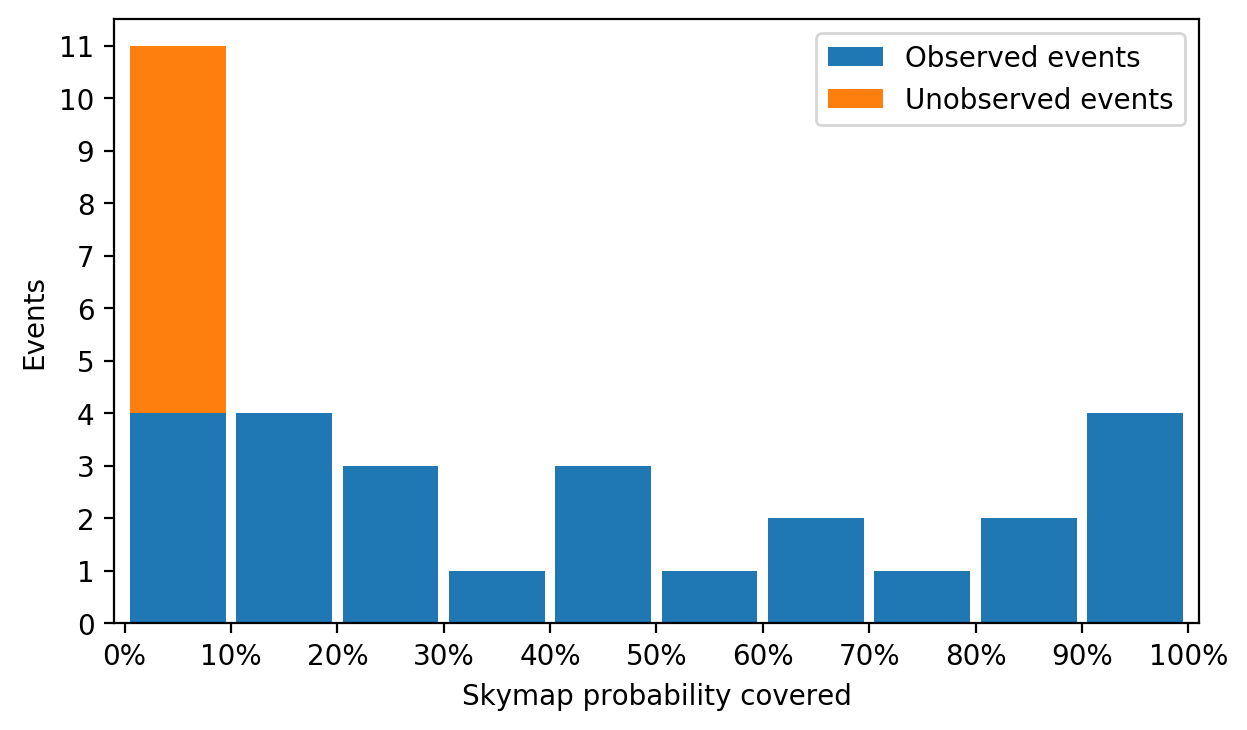
\includegraphics[width=0.95\linewidth]{images/events_prob.png}
    \end{center}
    \caption[Histogram of probabilities covered for O3 events]{
        Histogram of the skymap probability covered by GOTO for O3 events. \\
        7 of the 32 events were never observed (see \aref{tab:obs_log}).
    }\label{fig:events_prob}
\end{figure}

\begin{figure}[p]
    \begin{center}
    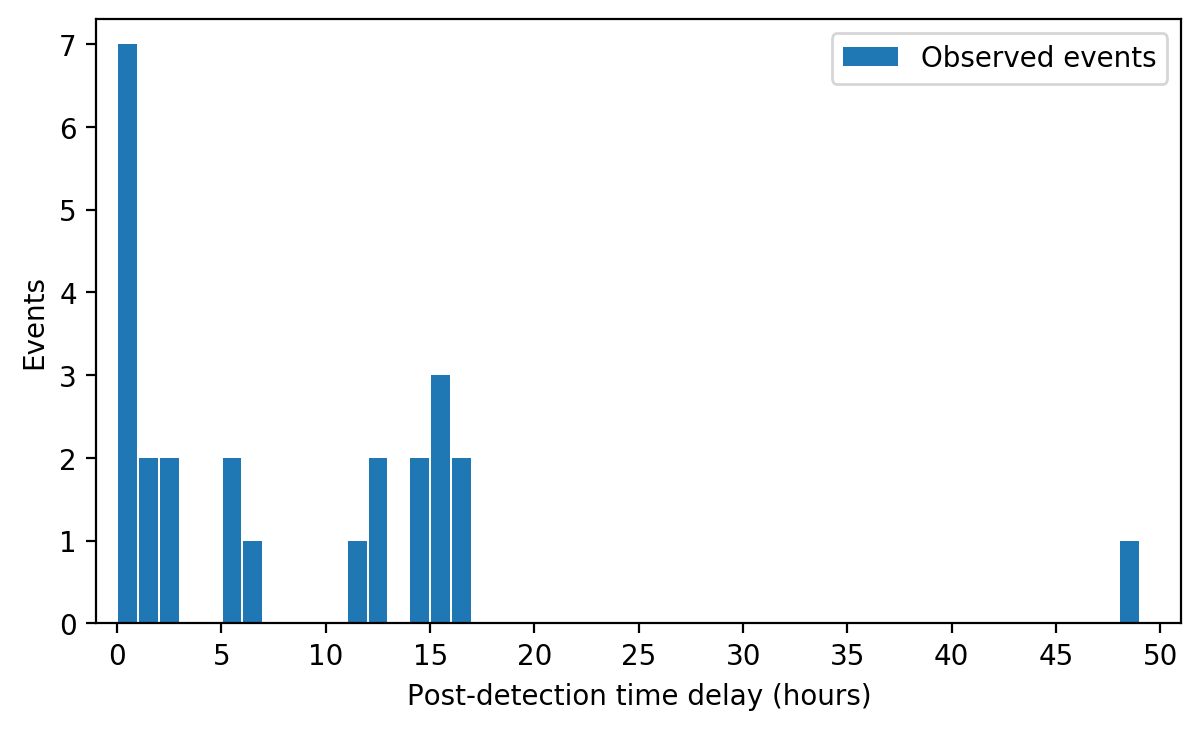
\includegraphics[width=0.95\linewidth]{images/events_delay.png}
    \end{center}
    \caption[Histogram of post-event delay for O3 events]{
        Histogram of the delay between the GW signal being detected by the LVC and GOTO commencing observations for O3 events. Events that GOTO did not observe are excluded. The outlier is S190421ar (due to a delay sending out the alert).
    }\label{fig:events_delay}
\end{figure}

\clearpage

\aref{fig:events_prob} shows the percentage of each event skymap covered by GOTO.\@ These value will depend on a variety of factors: for a particular event if only a small fraction of the skymap is covered that might be because of the position of the skymap in the sky, or a period of bad conditions forcing the dome to close. The coverage level is relatively even across all the events, once the seven events that GOTO did not observe are removed. \aref{fig:events_delay} shows the delay between the event being detected by the gravitational-wave detectors (from \aref{tab:gw_log}) and GOTO starting observations (from \aref{tab:obs_log}). For seven events GOTO was able to start observing less than an hour after the event was detected. This value includes factors such as the delay between the event being detected and the LVC releasing their alert, which was the cause for observations of S190421ar being delayed so long (see \aref{sec:challenges}). For this reason the time delay between the alert being received by the G-TeCS sentinel and the start of observations (given in \aref{tab:obs_log}) is a better indicator of the performance of the G-TeCS software.

Eight alerts were received while it was night time on La Palma, and the GOTO-alert event handling system allowed the pilot to immediately begin observations of the visible skymap. As shown in \aref{tab:obs_log}, in all but one of the eight cases the first exposure was started less than \SI{60}{\second} after the sentinel received the alert. The time delay varies between 28 and 56 seconds, primarily depending on how far the mount had to slew from its previous target. Of the remaining $\sim$\SI{25}{\second} delay, a significant amount is due to having to download the LVC skymaps, with the rest due to various small delays in the event handler, sentinel and pilot, such as the pilot needing to wait up to \SI{10}{\second} for the next scheduler check (see \aref{sec:checks}). Future optimisation could potentially reduce these delays further. The one exception was event S190513bm, which was immediately visible but observations were delayed by 4 minutes. At the time the alert was received the pilot was already observing a pointing from the S190512at event received the previous day; as both events were black hole binaries they were inserted at the same rank, and, as detailed in \aref{sec:toos}, equal-rank ToO pointings will not interrupt each other, so the new pointing had to wait until the previous one was completed. In all other cases the pilot was observing a lower-rank target, usually a survey tile, which was immediately aborted when the scheduler check returned the ToO gravitational-wave pointing.

\begin{table}[t]    \begin{center}
        \begin{tabular}{l|ccccc} % chktex 44
                                       & Post-detection   & Probability &  Area covered & $5\sigma$ limiting & GOTO \\
            \multicolumn{1}{c|}{Event} & time delay       & covered     & (sq deg)      & magnitude          & GCN \\
            \midrule
                             S190425z  & \SI{12.3}{\hour} & 22.6\%      & 2857          & $g=20.1$           & 24224 \tablefootnote{~~\citet{S190425z_GOTO}} \\
                             S190426c  &  \SI{5.3}{\hour} & 55.6\%      &  841          & $g=19.9$           & 24291 \tablefootnote{~~\citet{S190426c_GOTO}} \\
                             S190814bv &  \SI{1.8}{\hour} & 95.4\%      &  811          & $g=18.9$           & 25337 \tablefootnote{~~\citet{S190814bv_GOTO}} \\
        \end{tabular}
    \end{center}
    \caption[GOTO follow-up results for three key O3 events]{
        GOTO follow-up results for three key O3 events.
    }\label{tab:events_3key}
\end{table}

The three events that were the most likely to have a potential electromagnetic counterpart (originating from either a binary neutron star or neutron star-black hole binary) were S190425z, S190426c and S190814bv. The GOTO response to each was reported in a public GCN Notice, and the key values are given in \aref{tab:events_3key}.

S190425z was the second detection of gravitational waves from a binary neutron star after GW170817 \citep{S190425z}. Unlike GW170817 however, the signal was only detected by a single detector, LIGO-Livingston (LIGO-Hanford was offline at the time, and while Virgo did detect a signal it was below the valid signal-to-noise threshold). This resulted in a very large initial skymap, shown in \aref{fig:190425_goto}, with a 90\% contour area of 10,183 square degrees. Many other projects aside from GOTO followed-up this event, and the \acro{ztf} efforts were described in \aref{sec:followup}. Unfortunately a large portion of the skymap was located behind the Sun at the time and was therefore unobservable (on the right of \aref{fig:190425_goto}). The alert was received at 09:00 UTC, a few hours after GOTO had closed in the morning, meaning observations from La Palma could not begin for just over 12 hours until sunset that evening. The final skymap reduced the search area to 7,416 square degrees but shifted the probability even further into the unobservable region of the sky, meaning in the end GOTO only covered 22.6\% of the final probability.

\begin{figure}[t]
    \begin{center}
        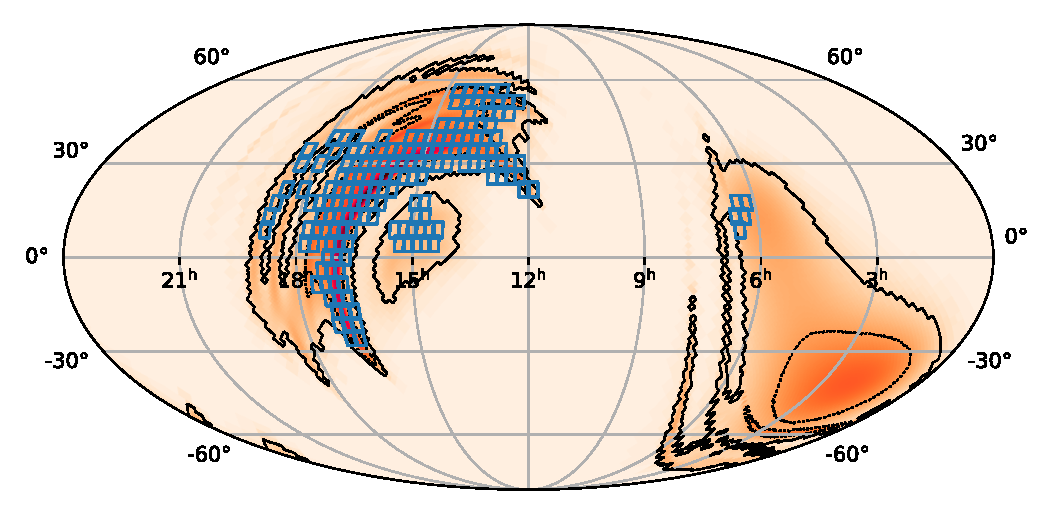
\includegraphics[width=0.9\linewidth]{images/190425_goto.pdf}
    \end{center}
    \caption[Follow-up observations of S190425z with GOTO]{
        GOTO follow-up observations of GW event S190425z \citep{S190425z_GOTO}. The tiled observations are shown in \textcolorbf{NavyBlue}{blue} over the initial skymap. Compare to \aref{fig:ztf}, which shows ZTF's coverage of the same event.
        }\label{fig:190425_goto}
\end{figure}

\begin{figure}[t]
    \begin{center}
        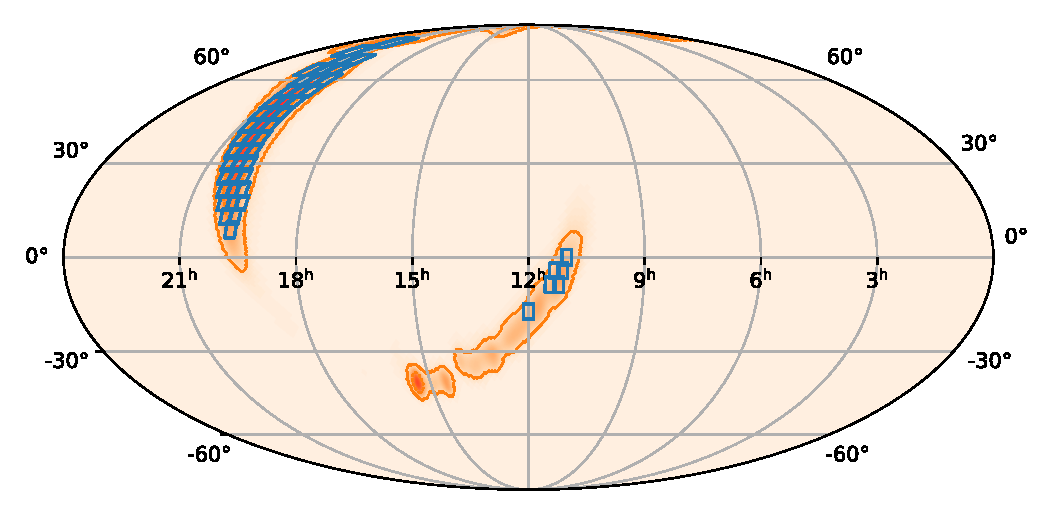
\includegraphics[width=0.9\linewidth]{images/190426_goto.pdf}
    \end{center}
    \caption[Follow-up observations of S190426c with GOTO]{
        GOTO follow-up observations of GW event S190426c \citep{S190426c_GOTO}. The tiled observations are shown in \textcolorbf{NavyBlue}{blue} over the initial skymap.
        }\label{fig:190426_goto}
\end{figure}

190426c was detected just 31 hours after S190425z \citep{S190425z}. This meant that on the night of the 26th GOTO was completing both the first pass of the 190426c tiles and the second pass of the S190425z tiles which had been first observed the previous night. The initial 190426c skymap and the tiles observed are shown in \aref{fig:190426_goto}. This time event was detected by all three detectors; the initial skymap had an area of 1,932 square degrees, and changed very little in the final skymap. The skymaps from the two events also did not overlap. Following-up two events at once had been considered in the design of the G-TeCS scheduling system (described \aref{chap:scheduling}), and as planned GOTO alternated between the two as tiles were observed (therefore lowering the effective rank as described in \aref{sec:rank}).

The latest event with a high chance of an optical counterpart was S190814bv \citep{S190814bv}, the first confirmed detection of gravitational waves from a neutron star-black hole binary. As shown in \aref{tab:gw_log} several other binary neutron star and neutron star-black hole binary events have been detected but have since been retracted. The initial skymap only included the contribution from the LIGO-Livingston and Virgo detectors, it covered 772 square degrees and is shown in \aref{fig:190826_goto}. A few hours later a revised skymap including LIGO-Hanford data was released, which reduced the 90\% contour region to just 38 square degrees. Unfortunately due to an error in how the LVC uploaded the skymap this was not immediately processed by GOTO (see \aref{sec:challenges}). The lower plot of \aref{fig:190826_goto} shows the GOTO tiles over the final skymap, and although a portion was below the observable horizon from La Palma GOTO still covered 95.4\% of the probability in just 5 pointings. The Moon was full at the time, hence the worse limiting magnitude in \aref{tab:events_3key}.

No electromagnetic counterparts were found for any of the three events, either by GOTO or other projects. But the G-TeCS follow-up code has proven to be fast and reliable, and GOTO will continue to follow-up LIGO-Virgo alerts. Based on the time from previous alerts, if, or when, another GW170817-like event is detected GOTO could potentially be observing the counterpart within seconds of the alert being received.

\newpage

% https://texfaq.org/FAQ-vertposfp
\makeatletter
\setlength{\@fptop}{0pt}
\makeatother

\begin{figure}[p]
    \begin{center}
        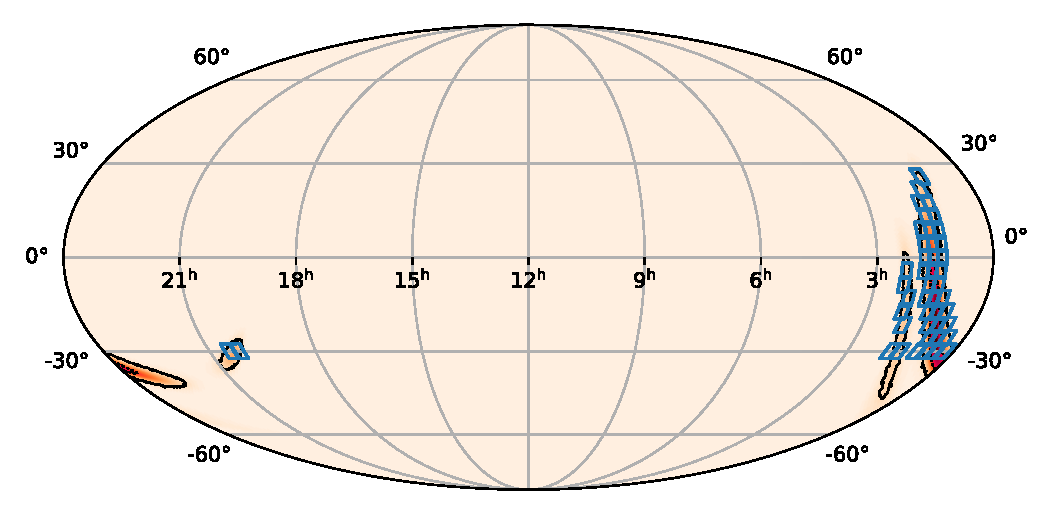
\includegraphics[width=0.9\linewidth]{images/190814_goto.pdf}
        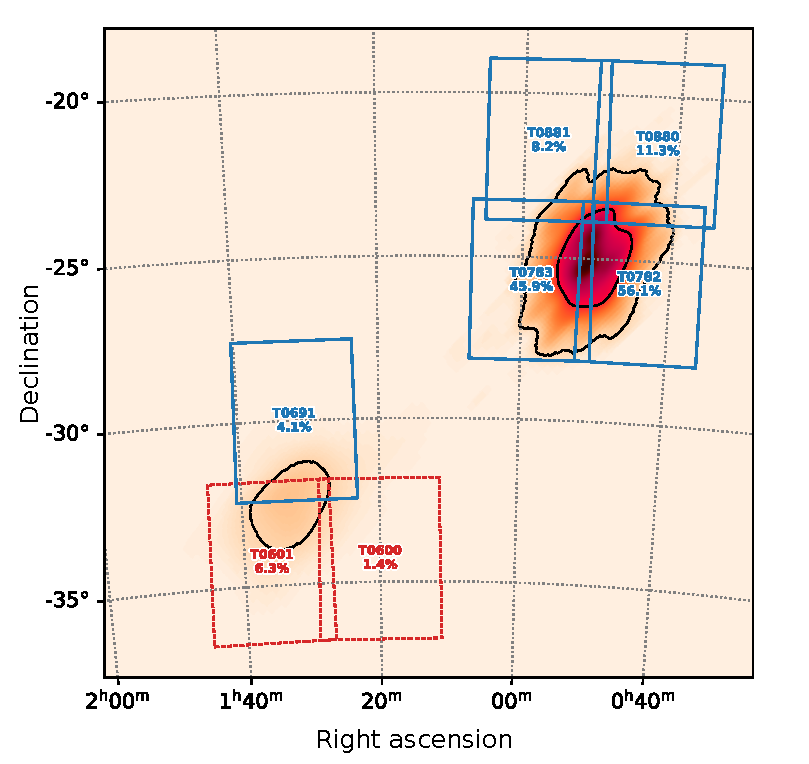
\includegraphics[width=0.8\linewidth]{images/190814_goto2.pdf}
    \end{center}
    \caption[Follow-up observations of S190814bv with GOTO]{
        GOTO follow-up observations of GW event S190814bv \citep{S190814bv_GOTO}. In the upper plot the tiled observations are shown in \textcolorbf{NavyBlue}{blue} over the initial skymap. The final skymap for this event is shown in the lower plot, with the seven GOTO tiles needed to cover the 90\% probability region. The two tiles in \textcolorbf{Red}{red} were below the local horizon and so were not observed.
        }\label{fig:190826_goto}
\end{figure}

\clearpage

% https://tex.stackexchange.com/questions/28556/how-to-place-a-float-at-the-top-of-a-floats-only-page
\makeatletter
\setlength{\@fptop}{0\p@ \@plus 1fil} % chktex 1
\makeatother

\newpage

\end{colsection}

% ########################################

\section{Future work}
\label{sec:future}

% ~~~~~~~~~~~~~~~~~~~~

\begin{colsection}

This thesis only details the beginning of the GOTO project, and the work described will need to be continued and built upon as the project expands in the future.

\end{colsection}

% ~~~~~~~~~~~~~~~~~~~~

\subsection{The global control system}
\label{sec:gtecs_future}
\begin{colsection}

Stage 1 of the GOTO project, the first mount and four unit telescopes, is currently observing from La Palma. The obvious direction of future work will be adapting and expanding G-TeCS in order to match the expansion of GOTO, as described in \aref{sec:goto_expansion}.

% ---------
\subsubsection{Stage 2}

Adding the second set of four unit telescopes to the existing mount on La Palma should require nothing more than a few configuration changes to handle the new interface daemons. On the scheduling side, the observation database will need to be reset with a new all-sky grid, based on the GOTO-8 field of view instead of the existing GOTO-4 tiles (see \aref{fig:fov}). As each tile will cover a larger area, the tile selection algorithm described in \aref{sec:mapping_skymaps} might need to be adjusted, and some of the observing strategy detailed in \aref{chap:alerts} could be revisited. Otherwise, no major changes are anticipated to be required, and the pilot should be able to resume observations immediately.

% ---------
\subsubsection{Stage 3}

The addition of the second mount in the second dome on La Palma will require more control system development. With two telescopes of the same design it should be simple to copy the hardware control daemons, and some systems could be shared between the two domes (for example, there is no need to have two conditions daemons both monitoring the same weather masts). A proposed system diagram is shown in \aref{fig:flow2}. But, as described in \aref{sec:multi_tel_scheduling}, the great benefit of having two telescopes is having them share a common scheduling system. This could be as simple as the system adopted for the multi-telescope simulations in \aref{chap:multiscope}, marking one telescope as the primary that always observes the highest-priority pointing and having the other always observe the second-highest. But in reality the telescopes will never be perfectly in sync, and there are more benefits to be gained from a more advanced scheduling system.

\begin{figure}[t]
    \begin{center}
        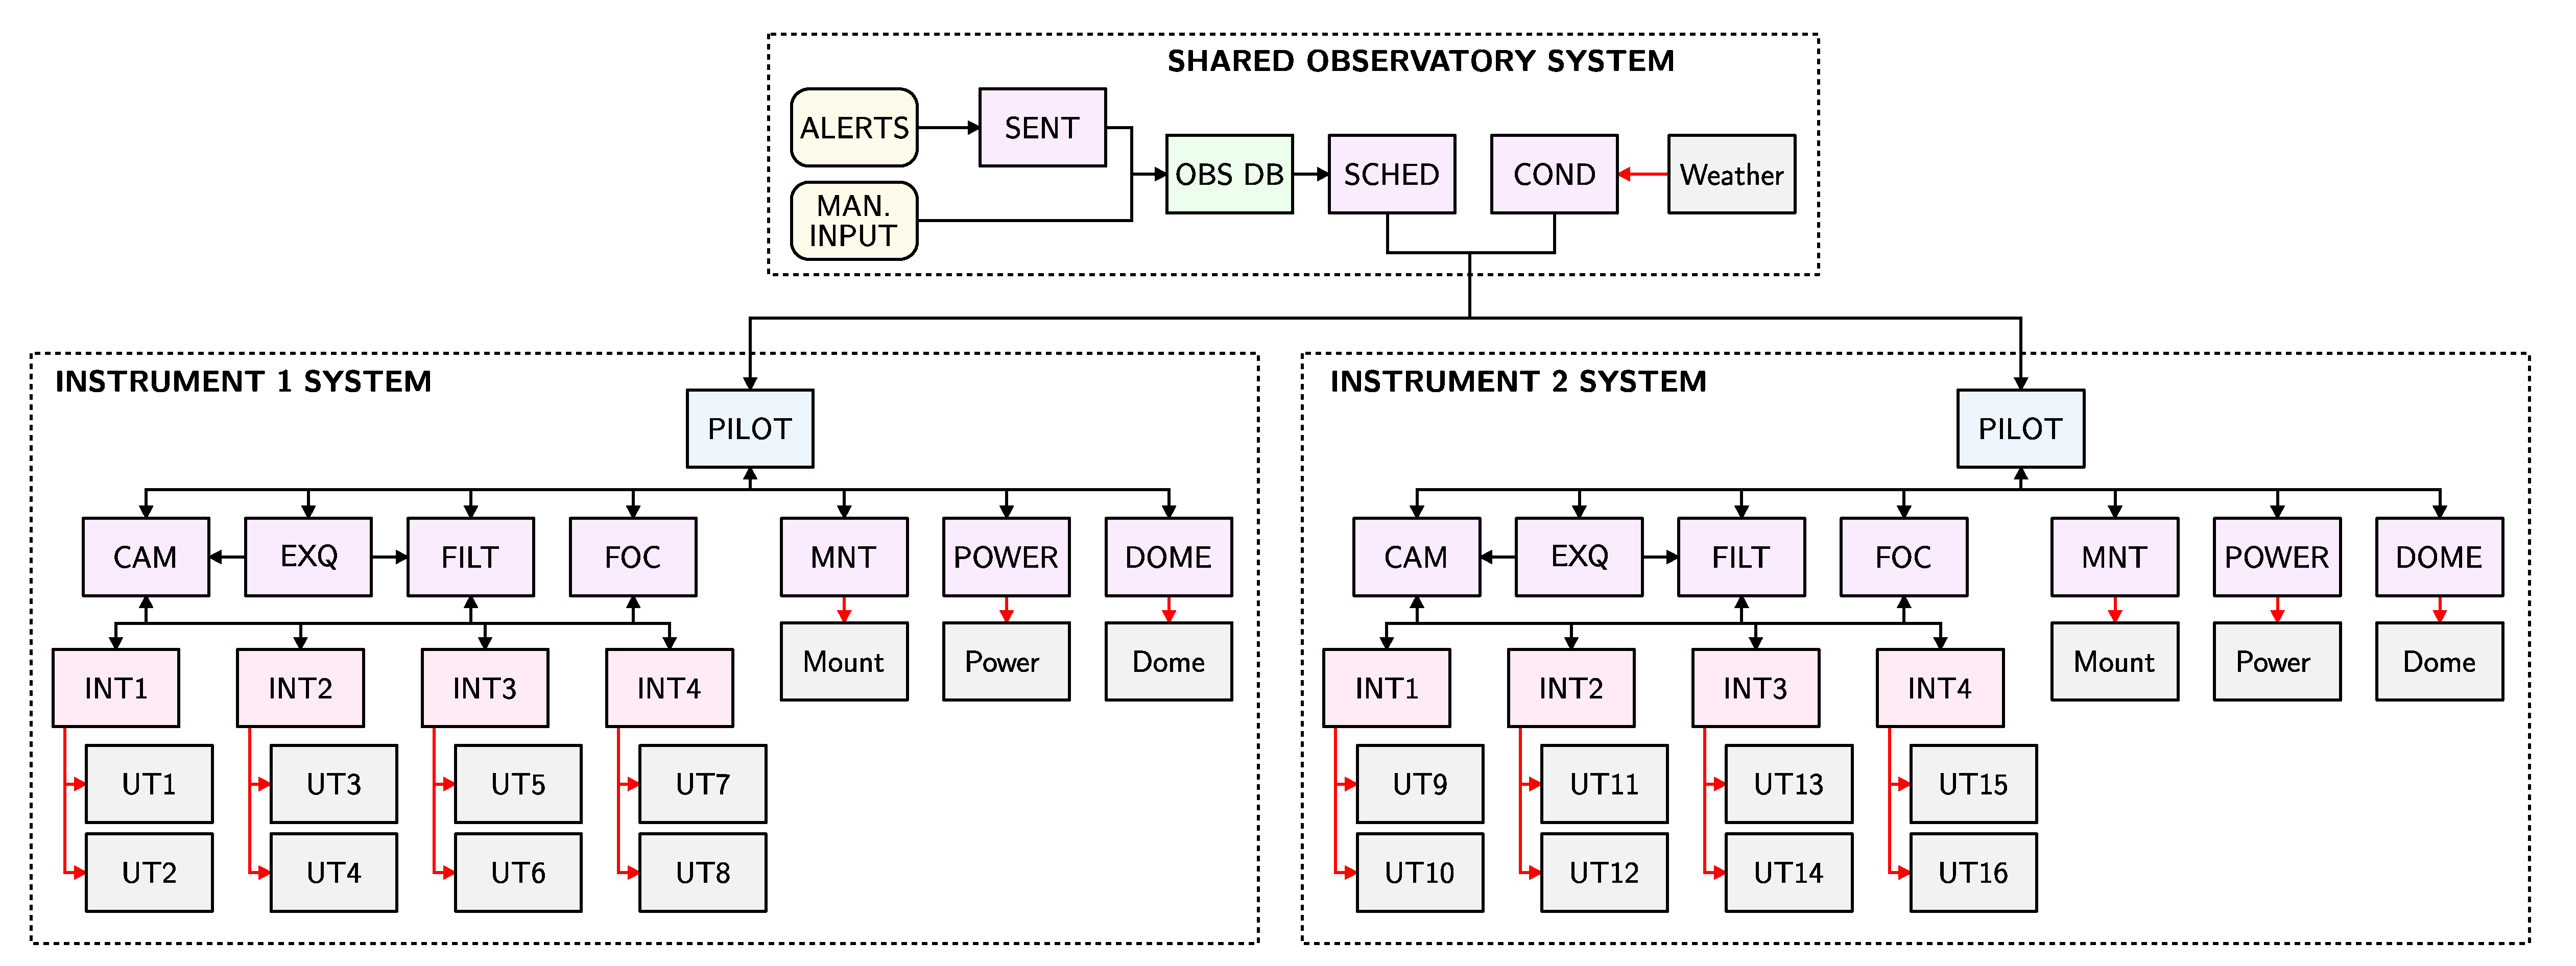
\includegraphics[width=\linewidth]{images/flow2.pdf}
    \end{center}
    \caption[Future G-TeCS system architecture for two telescopes]{
        Proposed future G-TeCS system architecture for controlling two telescopes at the same site (``Stage 3''). Note that the two pilots share the same scheduler and conditions daemons but are otherwise independent.
    }\label{fig:flow2}
\end{figure}

Just as the current scheduler described in \aref{chap:scheduling} has to decide what to observe based on various constraints, the next-generation scheduler will need to optimise which target is being observed by each telescope. Although several of the constraints will be the same for both mounts (e.g.\ the Moon phase or Sun altitude) it is possible that the two telescopes could have different artificial horizons and therefore altitude limits. The scheduler tie-breaking system will need to be revised, to account for distributing pointings to either telescope. One possible parameter to add to decide which telescope to send a pointing to would be the distance each mount would need to slew from the current target, and the scheduler could also account for the time left on the current observations (e.g.\ telescope 1 might be ready to observe while telescope 2 has 10 seconds left on the current target; if the difference in slew times to the new pointing is greater than \SI{10}{\second} then it would be better to wait for telescope 2 to finish).

The move from one 8-UT mount to two 8-UT mounts should mean the same all-sky grid can be used, as long as both have the same field of view (see \aref{sec:multi_grid_scheduling} for the problems inherent in observing with different grids). However, having multiple mounts opens up opportunities for more advanced observing strategies. They could both observe different parts of the sky to cover the survey or gravitational-wave skymaps more quickly, or they could observe the same tiles to achieve a greater depth when the images are stacked. The simulations in \aref{chap:multiscope} assumed coverage was the priority, but the future scheduling system should be designed to allow concurrent observations of the same tiles if required. The presence of the coloured filters adds even more possibilities. It should be possible to have the two telescopes observe the same target simultaneously but using different filters, to get immediate colour information on any sources. It might also be desirable to accept the impact on survey cadence and have each telescope carry out an independent survey in different filters, or perhaps have one taking rapid \SI{60}{\second} exposures while the other surveys the sky more slowly using the meridian scanning method detailed in \aref{sec:survey_sim_meridian}. The possibilities are endless, and although the ultimate decision will be made depending on the science requirements of the GOTO collaboration, ideally the future G-TeCS scheduling system should be able to handle whatever strategy is desired.

% ---------
\subsubsection{Stage 4}

The final form of the GOTO project is intended to include multiple telescopes at different sites across the globe. This is unlikely to happen before the second mount is built on La Palma, so by the time an Australian site is added the advanced systems described under Stage 3 above should already be in place, and ideally the next-generation scheduler should be able to delegate observations to multiple telescopes wherever they are in the world. There are several existing projects that operate in this manner which GOTO can emulate, such as the \acro{lco} network \citep{LCO_scheduling}.

\newpage

\end{colsection}

% ~~~~~~~~~~~~~~~~~~~~

\subsection{Continued development}
\label{sec:software_future}
\begin{colsection}

The work described in \aref{sec:gtecs_future} will be important to carry out as GOTO expands, but the timescales on which it will be needed will be dictated by the hardware status of the project. There is still plenty of software development work to do that is less dependent on the GOTO funding situation.

% ---------
\subsubsection{Pipeline integration}

One particular area of importance is better integration between the control system and the analysis pipeline and candidate marshal described in \aref{sec:gotophoto}. To achieve a fully autonomous system, the pipeline should be able to reschedule observations independently, for example if an image is affected by clouds. More excitingly, a future transient detection algorithm might be permitted to automatically schedule follow-up observations of promising candidates.

% ---------
\subsubsection{Unifying scheduler targets}

The scheduler system described in \aref{chap:scheduling} works well for both the all-sky survey and gravitational-wave follow-up events, as discussed in \aref{sec:conclusion}. However, one aspect that could be improved is the integration of both roles. For example, observing a particular tile as part of a gravitational-wave follow-up survey should be counted within the observation database as an observation of that tile for the all-sky survey as well, assuming they use the same filter. The GOTOphoto difference imaging pipeline already looks for reference images for difference imaging in all prior observations of that tile, regardless of what purpose it was taken for. In other words, observing tiles as part of a gravitational-wave skymap should also count towards the all-sky survey cadence: the same tiles are being observed, just in a different order.

\newpage

Another proposed addition in the same vein is linking tile observations between events. It is not uncommon for the same gamma-ray burst event to be detected by both \textit{Fermi} and \textit{Swift}; as described in \aref{sec:event_strategy}, both alerts are processed by the GOTO-alert event handler, and the only difference is that \textit{Swift} events are inserted into the observation database at a higher rank. This is intentional, as \textit{Swift} events typically are very well-localised, easily within a single GOTO tile, while the large skymaps for \textit{Fermi} events cover many tiles (see \aref{sec:grb_skymaps}). Because of this, if the sentinel detects an alert from both facilities within a few minutes, and the two skymaps overlap, then covering the large \textit{Fermi} skymap should be unnecessary, as the event source should be given by the much better localised \textit{Swift} position.

Independent detections of gamma-ray bursts are a common-enough example to test this behaviour, but where it could be very useful to GOTO is for coincident GRB and gravitational-wave events. The GW170817 event was notable as being also detected by \textit{Fermi} as GRB 170817A \citep{GW170817_Fermi}, and the LVC is investigating putting out automated alerts for future coincident GW-GRB events using the RAVEN pipeline \citep{RAVEN, LVC_userguide}. Were the G-TeCS sentinel able to achieve a similar result, simply prioritising GW skymap tiles that overlap with the GRB skymap, it could reduce the delay before observing the all-important tile that contains the counterpart kilonova.

% ---------
\subsubsection{Further simulations}

The test code written to simulate GOTO observations was a vital tool for optimising the G-TeCS scheduler (see \aref{sec:scheduler_sims}), and in \aref{chap:multiscope} it was used to model the benefits of GOTO's plans for future expansion. As described in \aref{sec:scheduler_sim_future}, it would be good to revisit the scheduler simulations with the benefit of subsequent code development and more-realistic simulation parameters based on the live GOTO system. Other scheduler simulations have also been proposed, for example to find optimal tile-selection limits for gravitational-wave skymaps (see \aref{sec:selecting_tiles}). A majority of the future work proposed in this chapter will also require further simulations, and making the simulation code as realistic as possible is a priority.

% ---------
\subsubsection{Code generalisation and availability}

Another potential future project that is being considered is the generalisation of some or all of the G-TeCS code, removing the GOTO-specific parts and making it usable by other projects. For example, the GOTO-tile code for creating survey grids and mapping skymaps to them described in \aref{chap:tiling} is not at all GOTO-specific, and would only require a small amount to work to rewrite into a separate Astropy-compatible Python package (probably along with a new name). On a wider scale, the G-TeCS control system could be adapted for other telescopes. A parallel version is already being used by the other Warwick telescopes on La Palma, and using G-TeCS is also being considered for other robotic telescope projects, such as the SAMNET solar telescope network \citep{SAMNET}. Currently all GOTO code is private, restricted only to GOTO collaboration members. However, if my code was reconfigured to be usable by other projects I would hope to make it publicly available and open-source.

\bigskip

Overall the GOTO Telescope Control System is still under active development, and this will continue as the GOTO project evolves. Based on the initial results from O3 the system has been working well and fulfilling its requirements, and it is therefore most likely only a matter of time until GOTO observes its first gravitational-wave counterpart.

\end{colsection}

% ########################################
